\section{Incorporating existing detector components into ProtoDUNE-ND}
\label{sec:MINERvA}
\todo{MINOS ND should be included to. needed for most basic ArC response. also, needs to be part of initial proposal to Steve, NOT a secondary request - From Debbie}

The MINERvA experiment~\cite{minerva-nim}, which now controls and maintains the re-purposed MINOS near detector, is located in the MINOS ND hall in which ProtoDUNE-ND will be installed, and is due to complete its data-taking in spring--summer 2019. The collaboration is currently considering its detector decommissioning plan, and it has been suggested that components of these existing detectors could be repurposed for ProtoDUNE-ND. As discussed in Section~\ref{sec:protodune-nd}, all DUNE ND designs considered in Ref.~\cite{dune_ndcsg} include some fast scintillator component. In this section, we outline the possible uses of the MINERvA detector components, and consider potential detector physics studies that they would bring to ProtoDUNE-ND.

\subsection{Repurposing the MINERvA detector}
The MINERvA detector is shown in Figure~\ref{fig:minerva_detector}. For the purpose of the discussion in this section, we will assume that the steel shield, scintillator veto plane, helium vessel, and nuclear targets region will be removed. 
\begin{figure}[htb]
  \centering
  \subfloat[Front view] {\label{fig:minerva_detector_front}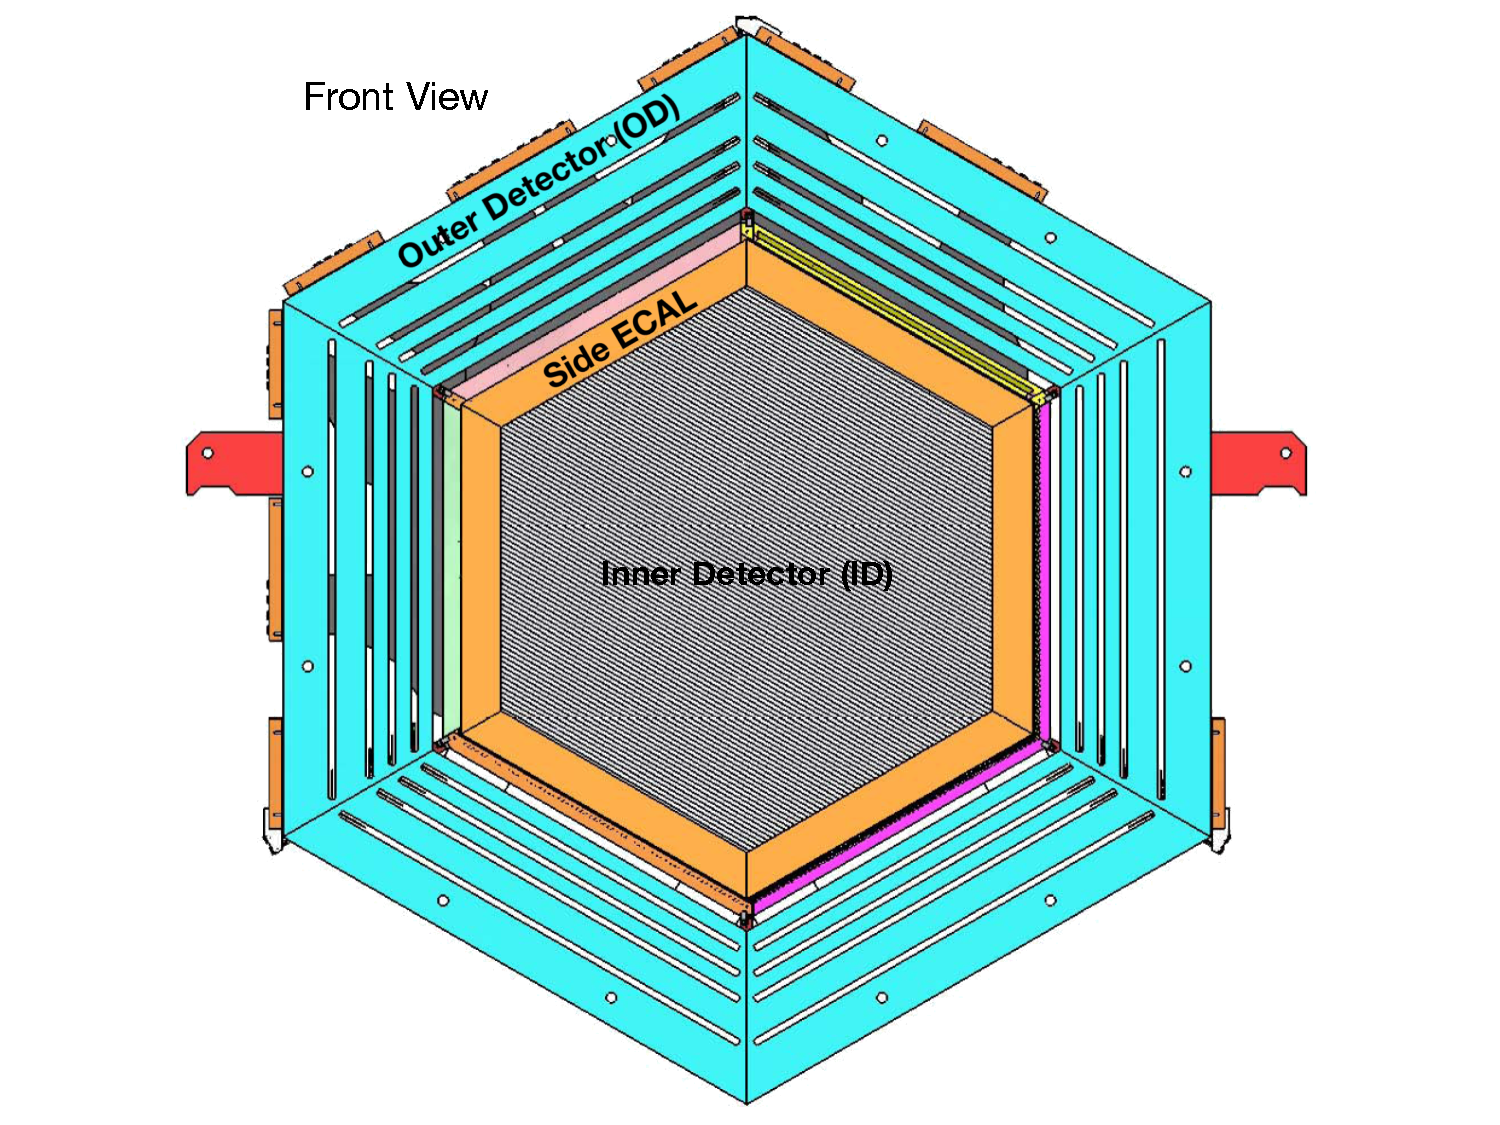
\includegraphics[width=0.35\textwidth]{plots/minerva_module_transverse}}
  \subfloat[Side view]  {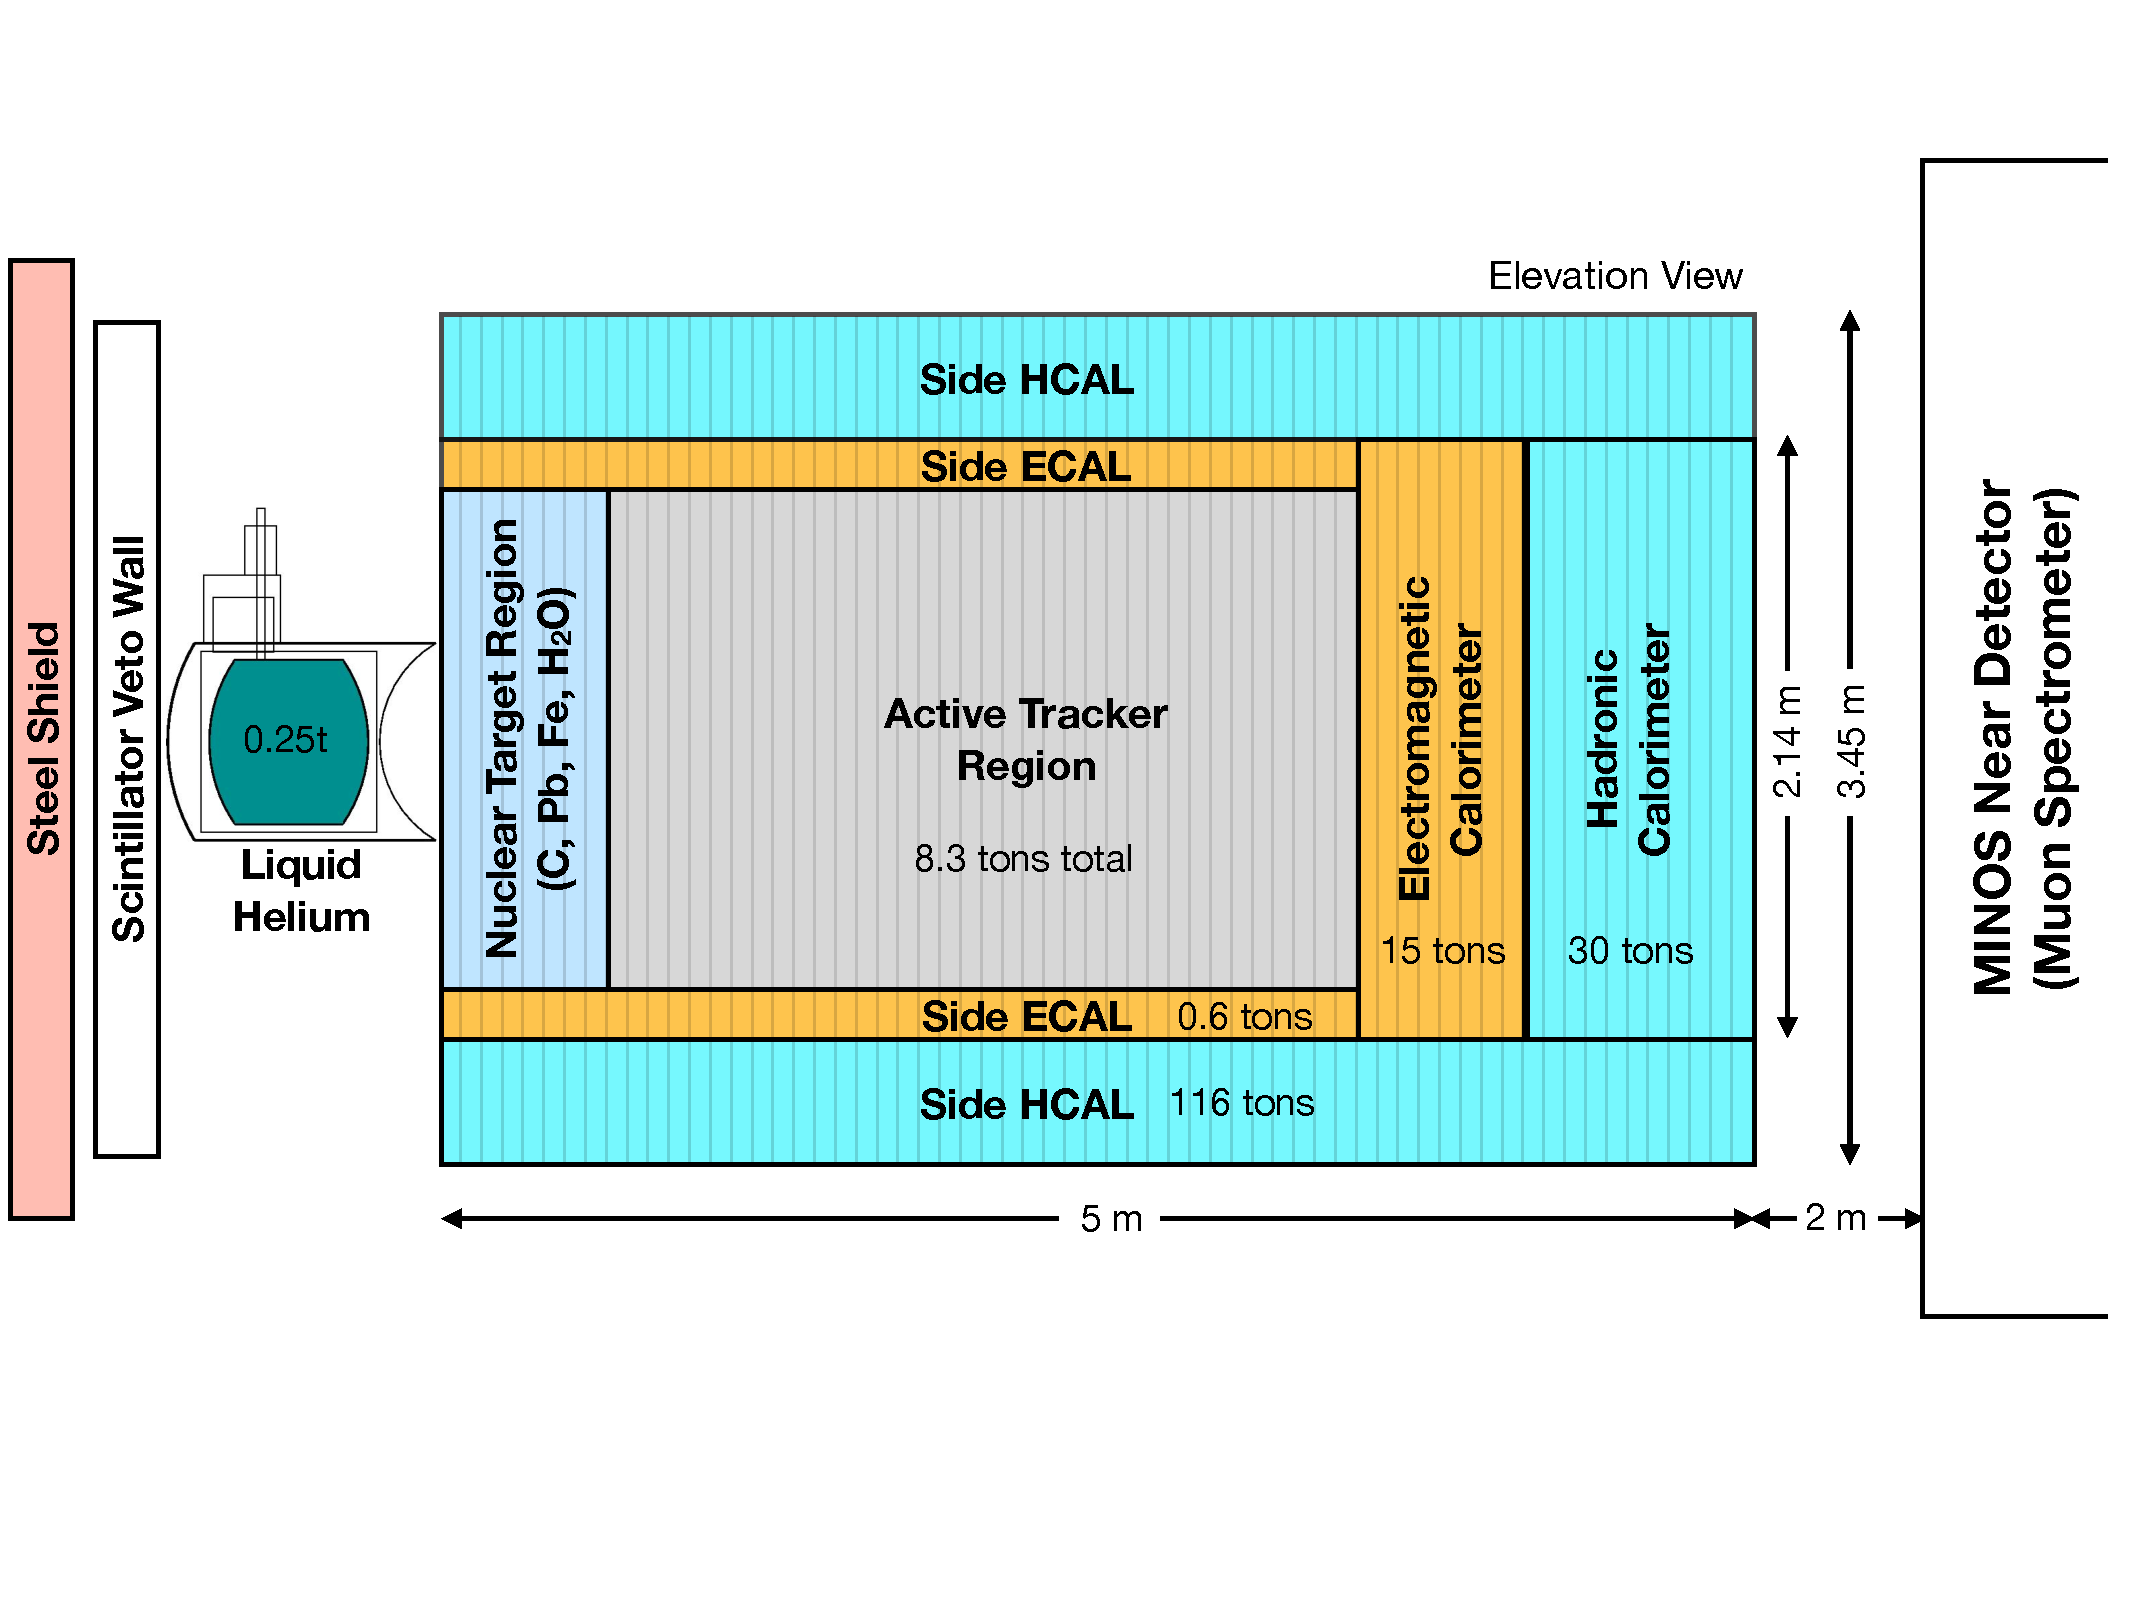
\includegraphics[width=0.60\textwidth]{plots/MINERvA_schematic.pdf}}
  \caption{Schematic of the MINERvA experiment. Reproduced from Figure 1 of Ref.~\cite{minerva-nim}.}
  \label{fig:minerva_detector}
\end{figure}

The remaining central tracking region, and both the electromagnetic(EM) and hadronic calorimeters are divided into modules which consist mostly of hexagonal scintillator planes, each made of 127 triangular scintillator bars, arranged in three different orientations (60$^\circ$ rotations between each plane). There are 62 modules in the fully-active tracker region, each composed of two scintillator layers. A 15 cm border of 0.2 mm thick lead on the downstream end of each module provides EM calorimetry for particles exiting the side of the tracking region.

The downstream EM calorimeter is composed of 10 modules, each with two scintillator planes and a 0.2 mm thick lead plate on the downstream end. There are 20 modules in the downstream hadronic calorimeter, each with a single scintillator plane and a 2.54 cm thick hexagonal steel plane. The outer detector consists of a steel frame supporting structure with embedded scintillator planes, as can be seen in Figure~\ref{fig:minerva_detector_front}, which turns the support structure into a hadronic calorimeter. The combination of the downstream and side EM and hadronic calorimeters allows for containment of most particles which escape from the central tracking region, and allows for particle identification and momentum measurements.

\begin{figure}[htb]
  \centering
  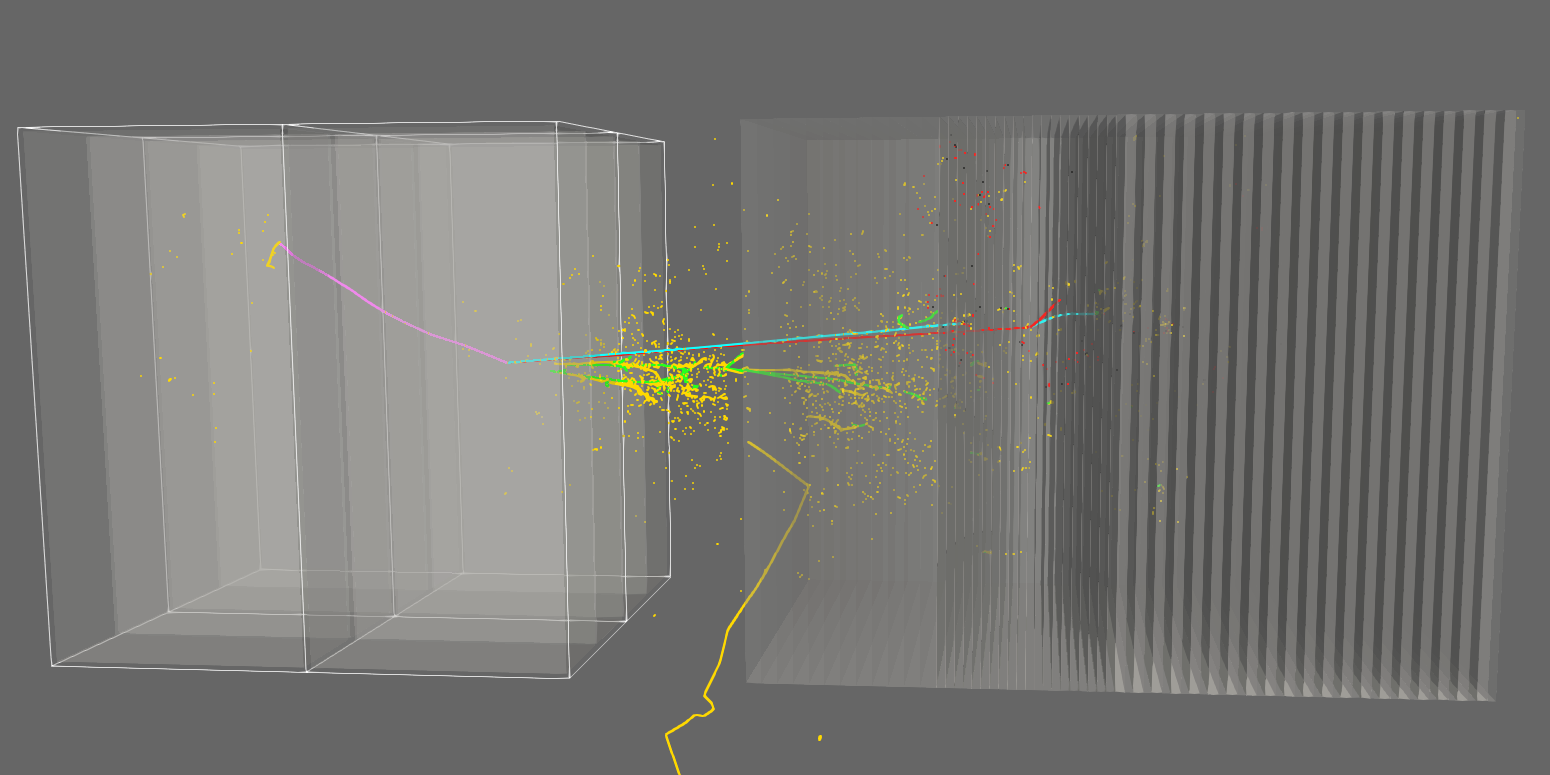
\includegraphics[width=0.8\textwidth]{{plots/Event_Displays_2x2_MINERvA/MINERvA_full_e70_rectangle_crop}.png}
  \caption{Example simulated event for a 7.0 GeV $\nu_{\mu}$--argon charged-current interaction, in which particles not contained in the ArgonCube 2x2 enter the MINERvA central tracking region downstream. Energy deposits are color-coded according to the particle type: $\pi^{\pm}$ --- blue; $\mu^{\pm}$ --- purple; $e^{+}$ --- green; $e^{-}$ --- yellow; proton --- red; recoiling nuclei --- black. The event vertex was randomly placed inside the active volume of the 2x2 Demonstrator module.}
  \label{fig:2x2+MINERvA_event}
\end{figure}
For the studies shown in this section, a simulation was performed approximating the downstream MINERvA central tracking region with a box of scintillator, and the ArgonCube 2x2 Demonstrator module upstream of the shortened MINERvA detector. \todo{Chris M to actually describe what this is...} An example event is shown in Figure~\ref{fig:2x2+MINERvA_event}, and can be compared with 2x2 only events in Figures~\ref{fig:argonbox_event_display} and~\ref{fig:leaky_event}. Note that this simulation only included the ArgonCube cryostat and MINERvA detector components, no material was included outside these (so escaping particles simply leave without ever re-interacting). This is unlike the previously described ArgonBox simulation, where a large box of argon was simulated (so escaping particles still re-interact). Events were again distributed uniformly throughout the ArgonCube active volume.

In the following, we discuss potential detector physics studies, or improvements to detector physics studies previously discussed in the ArgonCube 2x2-only case (in Section~\ref{sec:detector-physics-studies}), incorporating elements of the MINERvA detector downstream of the ArgonCube 2x2 module.

\subsubsection{Track matching}
All DUNE ND designs considered in Ref.~\cite{dune_ndcsg} include some fast scintillator component, downstream of the LAr ArgonCube component, and downstream of a low-density GAr TPC tracker, to tag escaping particles, photons, and possibly neutrons. There is a significant reconstruction challenge in matching the escaping tracks from the LAr component, with the signals in the scintillator, given the slow charge readout in the LAr TPC, and the high multiplicity DUNE-ND environment.

\begin{figure}[htb]
  \centering
  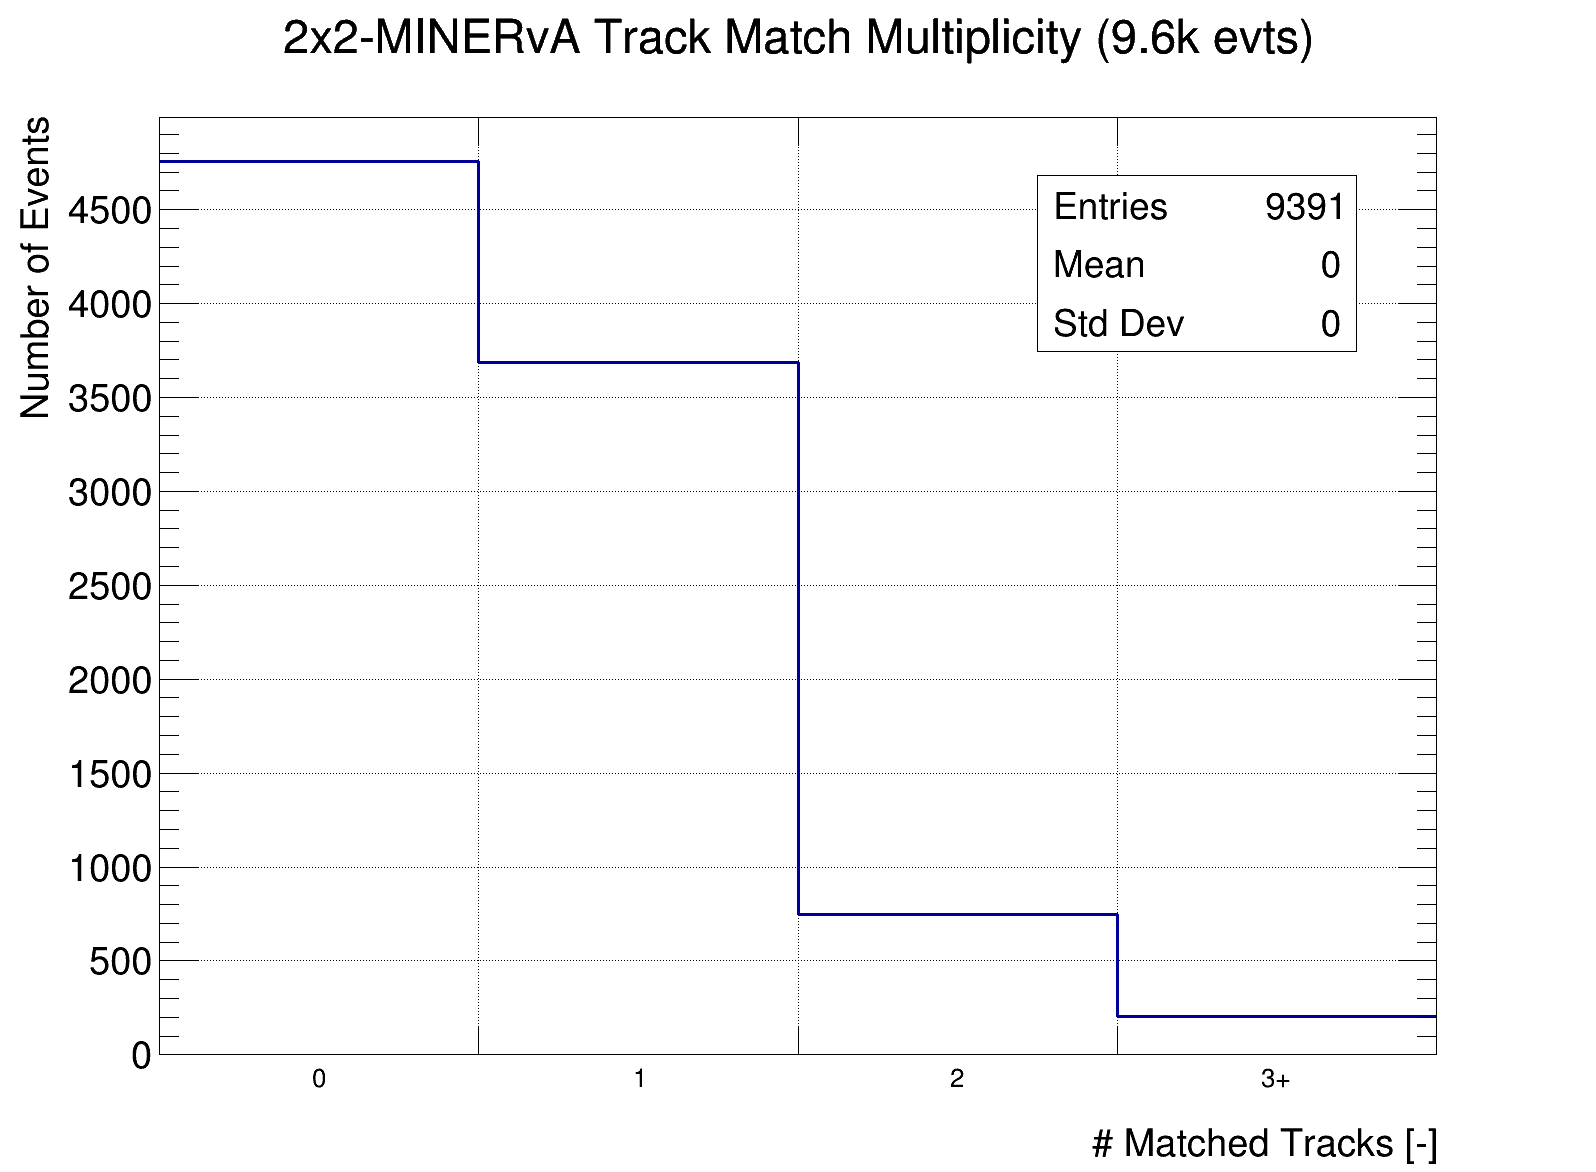
\includegraphics[width=0.45\textwidth]{plots/2x2_minerva_plots/track_mathch_multiplicity.png}
  \caption{Simulated number of true tracks produced by simulated GENIE interactions in the ArgonCube 2x2 active volume, which deposit energy in both the 2x2 module, and the MINERvA component positioned downstream of the 2x2.}
  \label{fig:track_multiplicity}
\end{figure}
Many tracks produced in the LAr volume are not contained by the ArgonCube 2x2 module, and the majority will escape downstream. In Figure~\ref{fig:hadronic_containment}, the multiplicity of tracks which deposit charge in both the ArgonCube 2x2 module and the MINERvA component, included in the simulation described above, are shown. Full DUNE-ND events are likely to have an even higher LAr to scintillator track multiplicity due to the pile-up in the much larger 35 t ArgonCube LAr detector. But it is clear from Figure~\ref{fig:track_multiplicity} that including MINERvA elements in the ProtoDUNE-ND tests would provide useful data with which to start tackling this reconstruction problem.

\begin{figure}[htb]
  \centering
  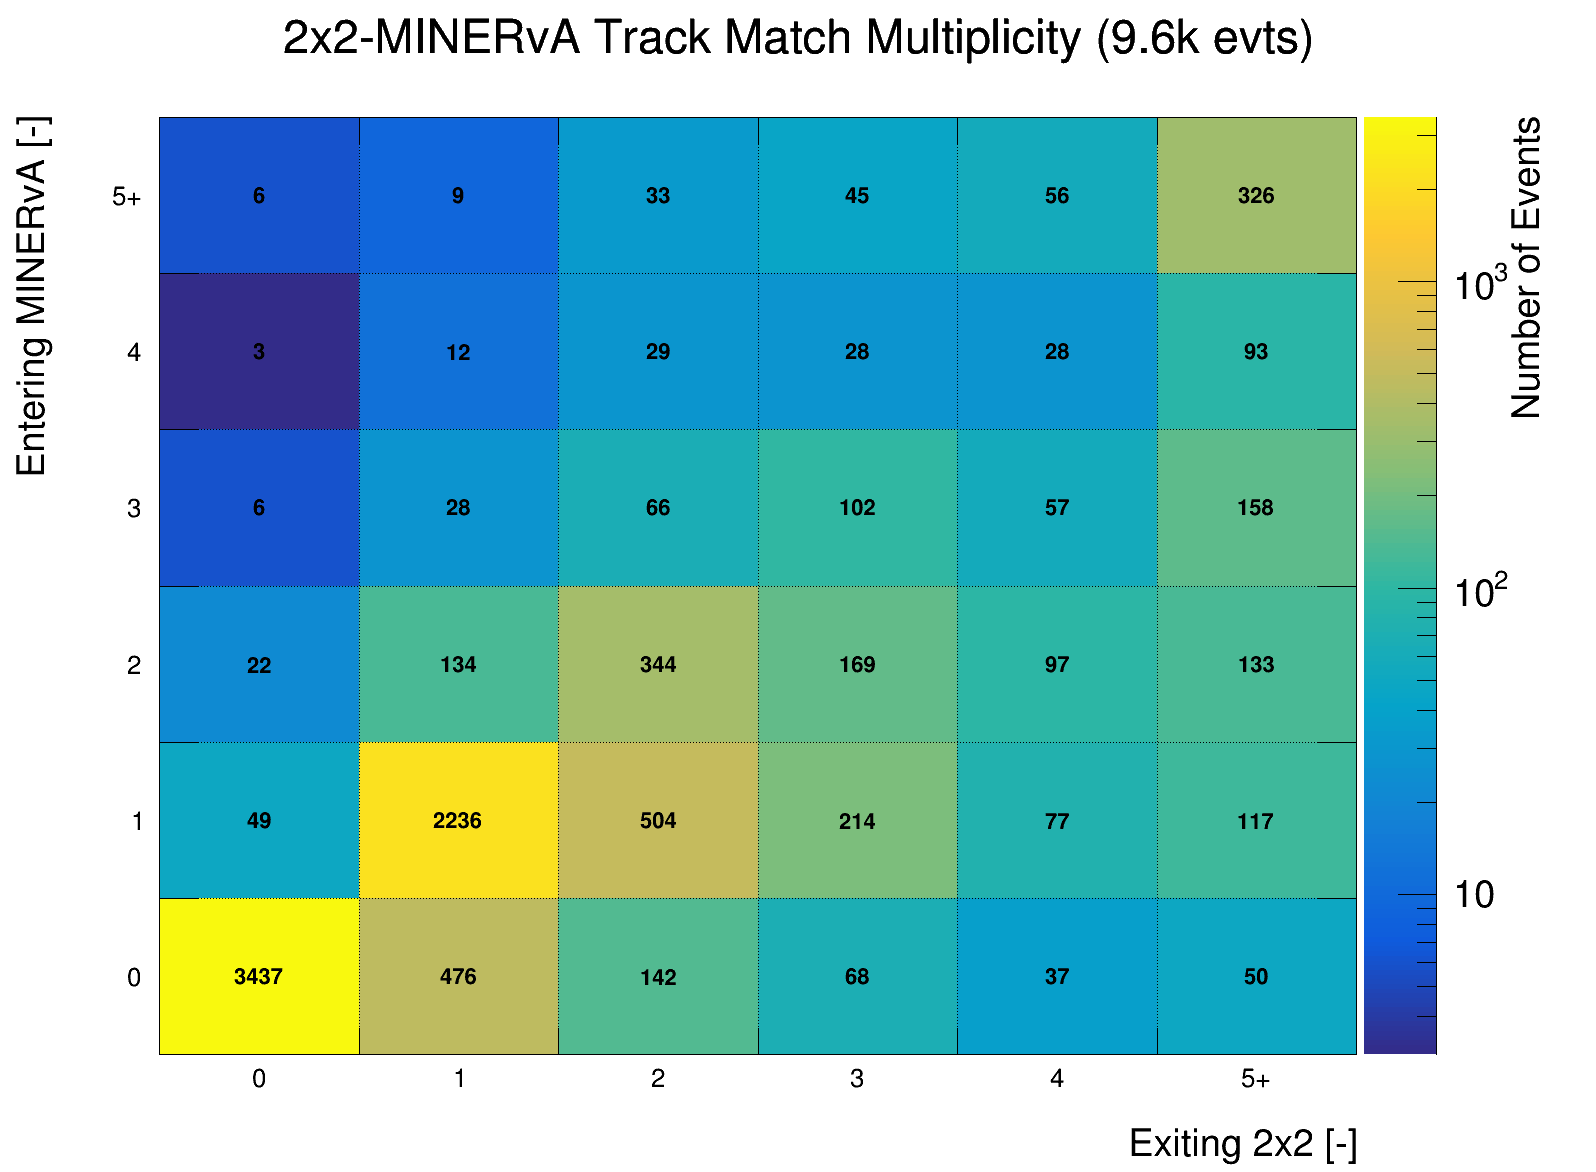
\includegraphics[width=0.45\textwidth]{plots/2x2_minerva_plots/track_mathch_topo.png}
  \caption{Simulated number of true tracks produced by simulated GENIE interactions in the ArgonCube 2x2 active volume, which exit the downstream face of the 2x2 module, relative to the number of tracks which enter the upstream face of the downstream MINERvA component, event by event.}
  \label{fig:track_multiplicity_topo}
\end{figure}
As can be seen from the event display shown in Figure~\ref{fig:2x2+MINERvA_event}, events in which tracks escaping the 2x2 active volume may re-interact in the surrounding LAr bath before entering the MINERvA component included in this simulation, thus making the event more confusing, and difficult to assess reconstruction performance with. Figure~\ref{fig:track_multiplicity_topo} shows the multiplicity of tracks exiting the downstream face of the 2x2 active volume downstream \todo{Patrick, this is the downstream face only right?}, compared with the number of tracks entering the upstream face of the MINERvA component included in the simulation. The distribution is fairly diagonal, suggesting that althoguh complicated event topologies exist, the events will not be too confused to use for these studies. Note also that this problem could be dramatically reduced by partially instrumenting the dead region between the two detectors.

\subsubsection{Acceptance studies}
\todo{Update with higher statistics}

The inclusion of MINERvA in ProtoDUNE-ND will improve the acceptance of particles for various studies. Here, we show how the efficiency for contained events compares for the 2x2+MINERvA setup desribed above, with MINERvA components located downstream of the ArgonCube 2x2 Demonstrator module, and for the 2x2-only case.

\begin{figure}[htb]
  \centering
  \subfloat[2x2-only]    {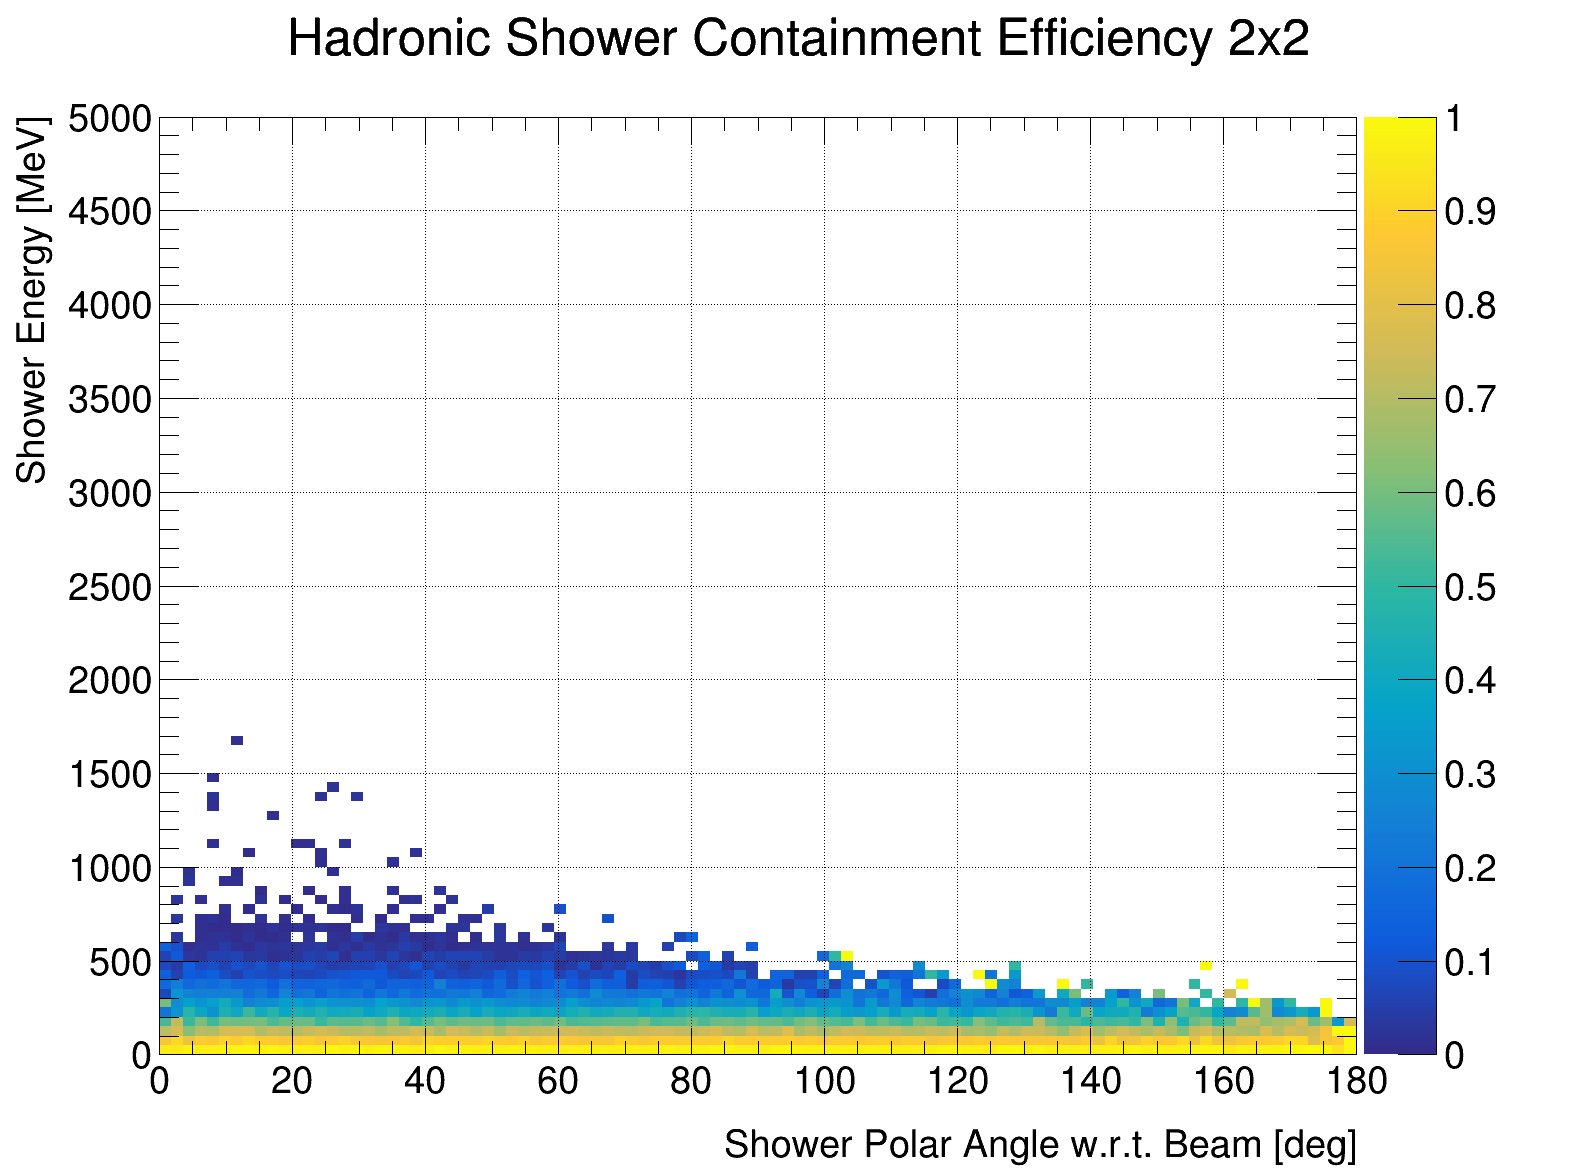
\includegraphics[width=0.45\textwidth]{plots/2x2_minerva_plots/H_cont_eff_2x2.png}}
  \subfloat[2x2+MINERvA] {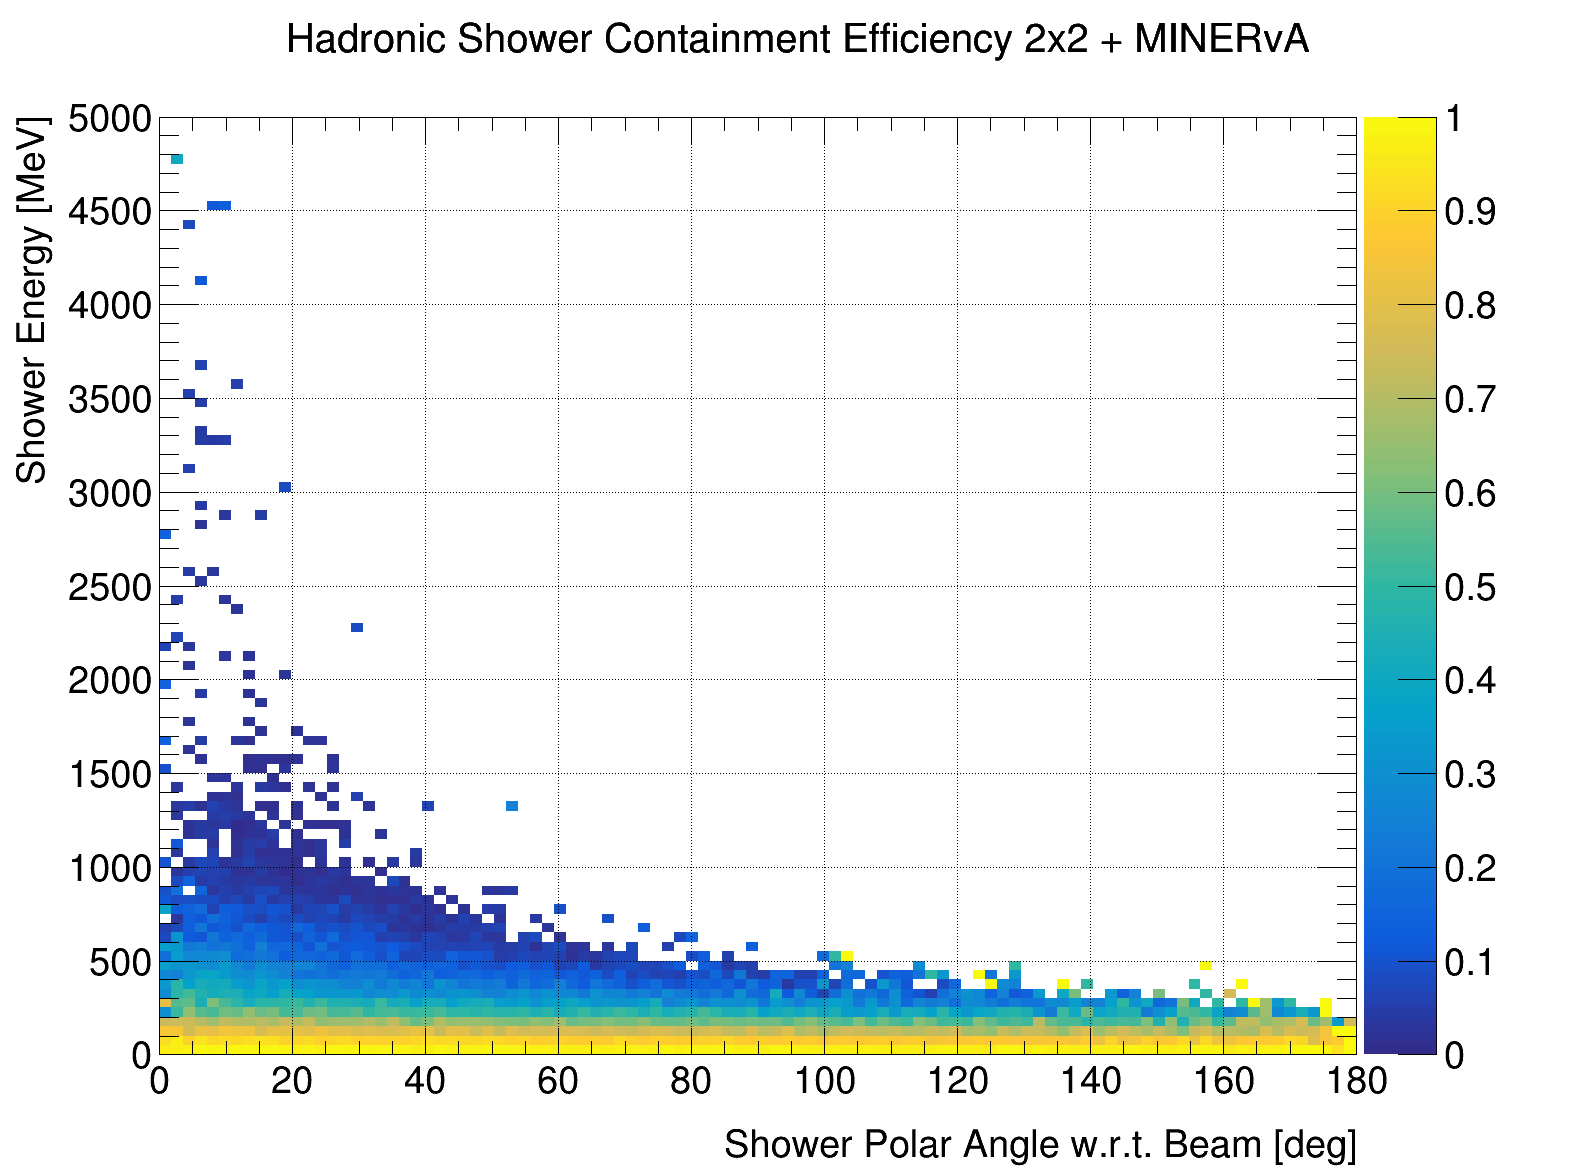
\includegraphics[width=0.45\textwidth]{plots/2x2_minerva_plots/H_cont_eff_2x2_MINERvA.png}}
  \caption{Efficiency for containing hadronic showers, in the 2x2-only, and 2x2+MINERvA, as a function of hadronic shower energy and angle w.r.t the incoming neutrino direction. Containment is defined as $\geq$90\% of the energy being deposited in an active volume of a detector.}
  \label{fig:hadronic_containment}
\end{figure}
In Figure~\ref{fig:hadronic_containment}, the containment of hadron-induced showers is shown as a function of the true energy of the shower, and its angle w.r.t the incoming neutrino beam direction. Showers are defined as being contained when $\geq$90\% of the true energy of the shower is deposited inside the active 2x2 volume, or the MINERvA component if applicable. As expected, including a MINERvA component downstream of the 2x2 module increases the efficiency for angles $\theta \lesssim 30^{\circ}$, which dramatically increases the containment of high energy $E \gtrsim 0.5$ GeV hadronic showers, which tend to be forward-going.

\begin{figure}[htb]
  \centering
  \subfloat[2x2-only]    {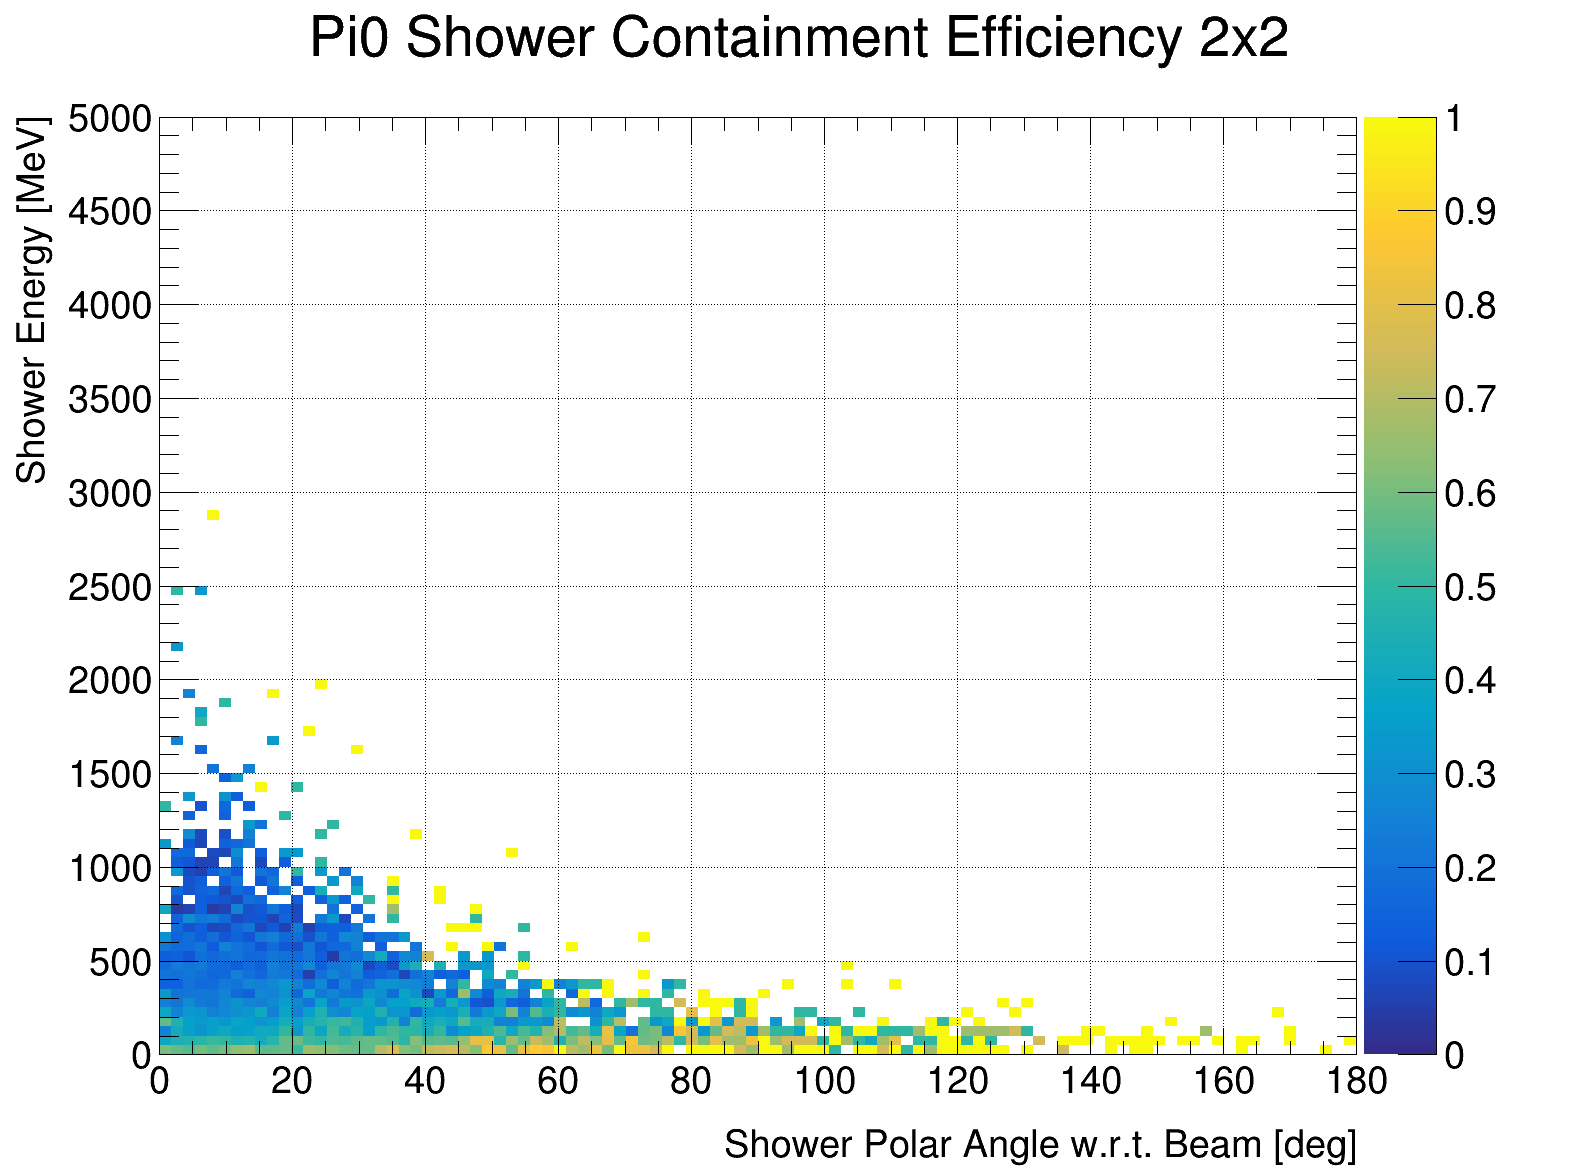
\includegraphics[width=0.45\textwidth]{plots/2x2_minerva_plots/Pi0_cont_eff_2x2.png}}
  \subfloat[2x2+MINERvA] {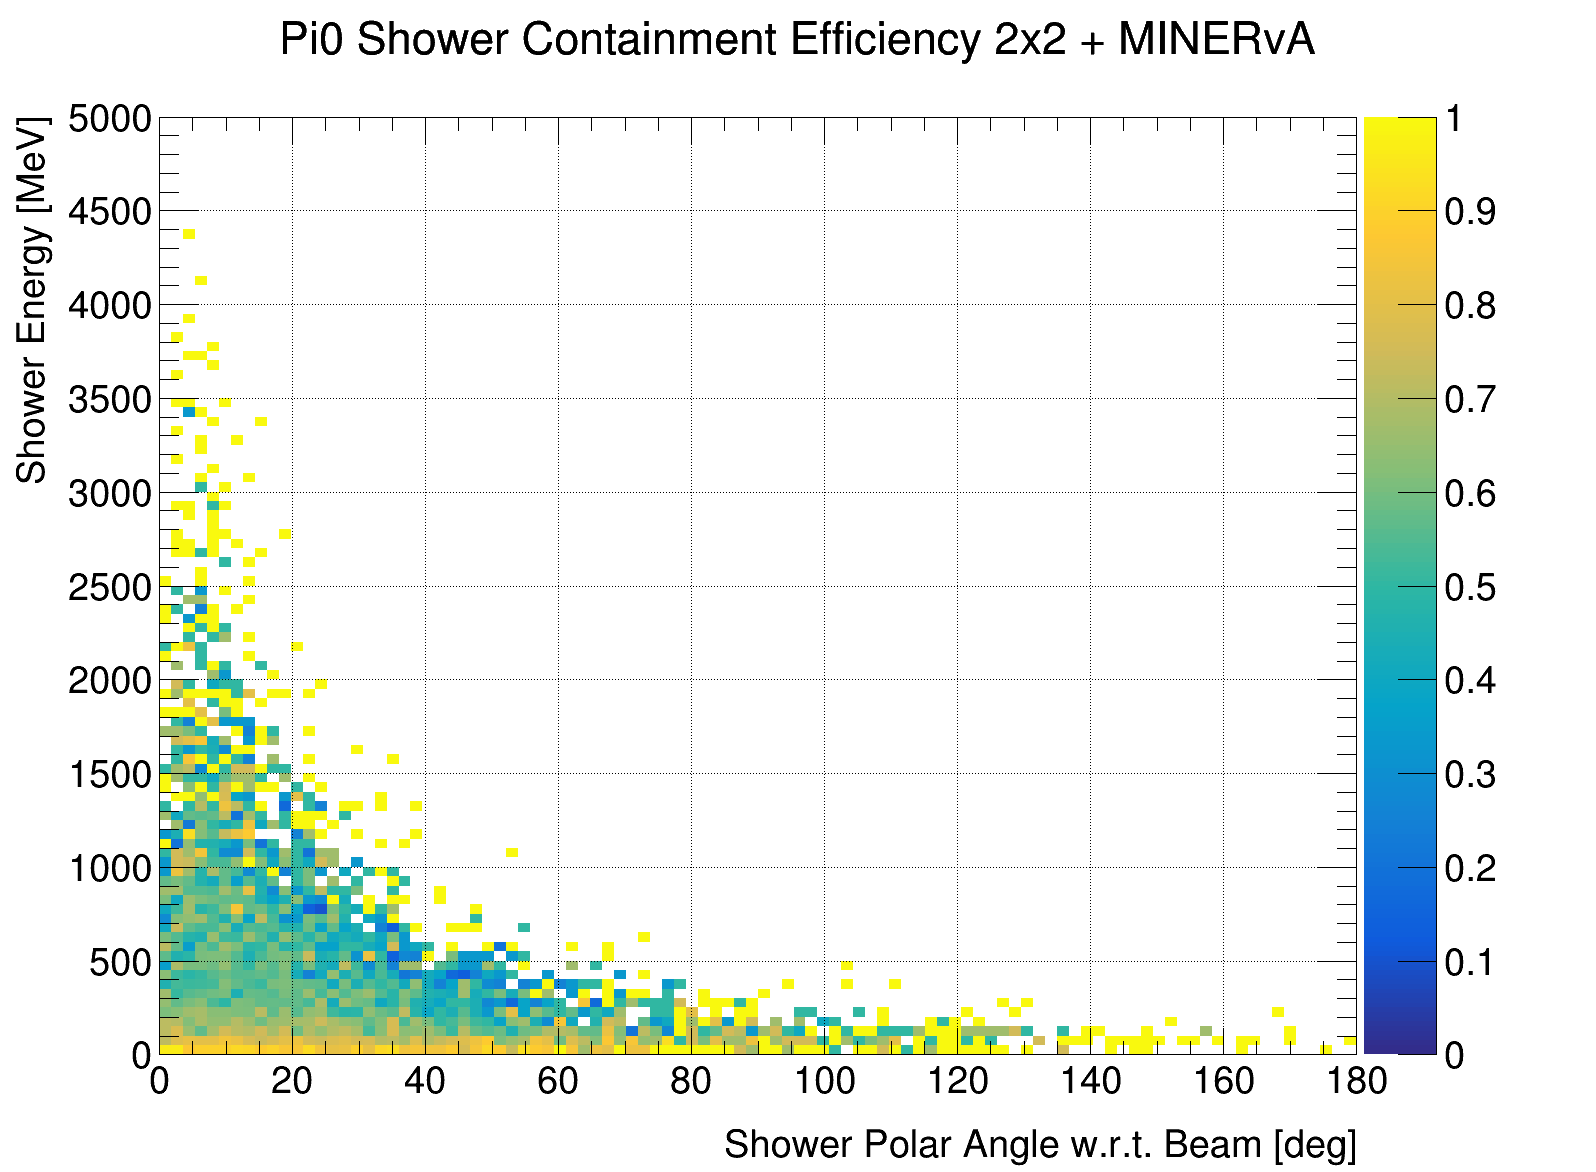
\includegraphics[width=0.45\textwidth]{plots/2x2_minerva_plots/Pi0_cont_eff_2x2_MINERvA.png}}
  \caption{Efficiency for containing both photo-induced showers from $\pi^{\circ}$ decays, in the 2x2-only, and 2x2+MINERvA, as a function of the $\pi^{0}$ kinetic energy and angle w.r.t the incoming neutrino direction. Containment is defined as $\geq$90\% of the energy being deposited in an active volume of a detector.}
  \label{fig:pi0_containment}
\end{figure}
As discussed previously in this note, as the 2x2 module will not be placed in a test beam prior to installation in the NuMI beam at Fermilab, measurements in which the energy scale of the 2x2 can be calibration will be vital to assess the quality of energy reconstruction in the detector. The containment of both photons from a $\pi^{0}$ decay provides an appropriate in situ measurment of the energy reconstruction capabilities. In Figure~\ref{fig:pi0_containment}, the efficiency to contain 90\% of the energy from both photon-induced showers from a $\pi^{0}$ decay within the active volume of the 2x2, or the MINERvA component if relevant, is shown as a function of the $\pi^{0}$ kinetic energy and angle w.r.t the incoming neutrino beam \todo{Patrick, check this}. There is a significant increase in efficiency for all kinetic energies above a few hundred MeV, particularly for high energy ($E_{\pi^{0}} \gtrsim 1$ GeV) pions, which are produced in the forward direction. Although the dead space between the ArconCube 2x2 active volume and the MINERvA component complicates this picture somewhat, it is clear that including a large portion of MINERvA would give much greater statistics for this benchmark test of the ArgonCube detector performance.

\subsubsection{Neutron tagging studies}


\begin{figure}[htb]
  \centering
  \subfloat[2x2]    {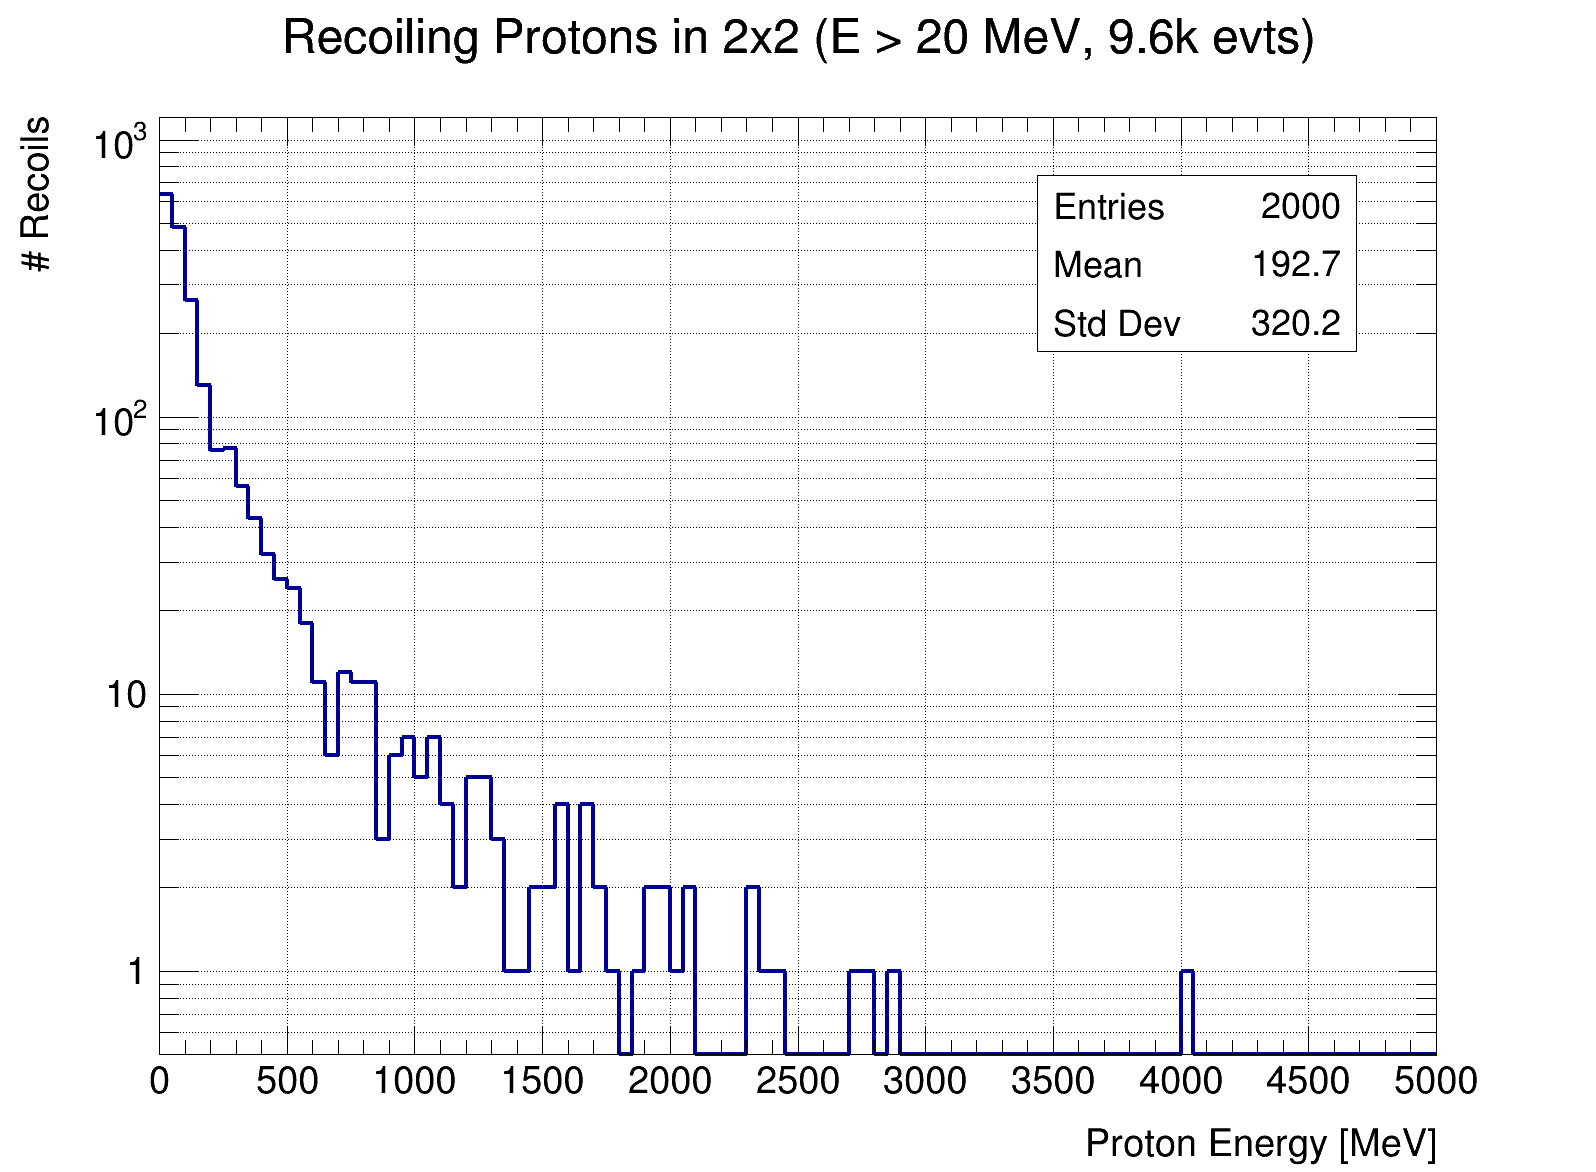
\includegraphics[width=0.45\textwidth]{plots/2x2_minerva_plots/recoils_vs_E_proton_2x2.png}}
  \subfloat[MINERvA] {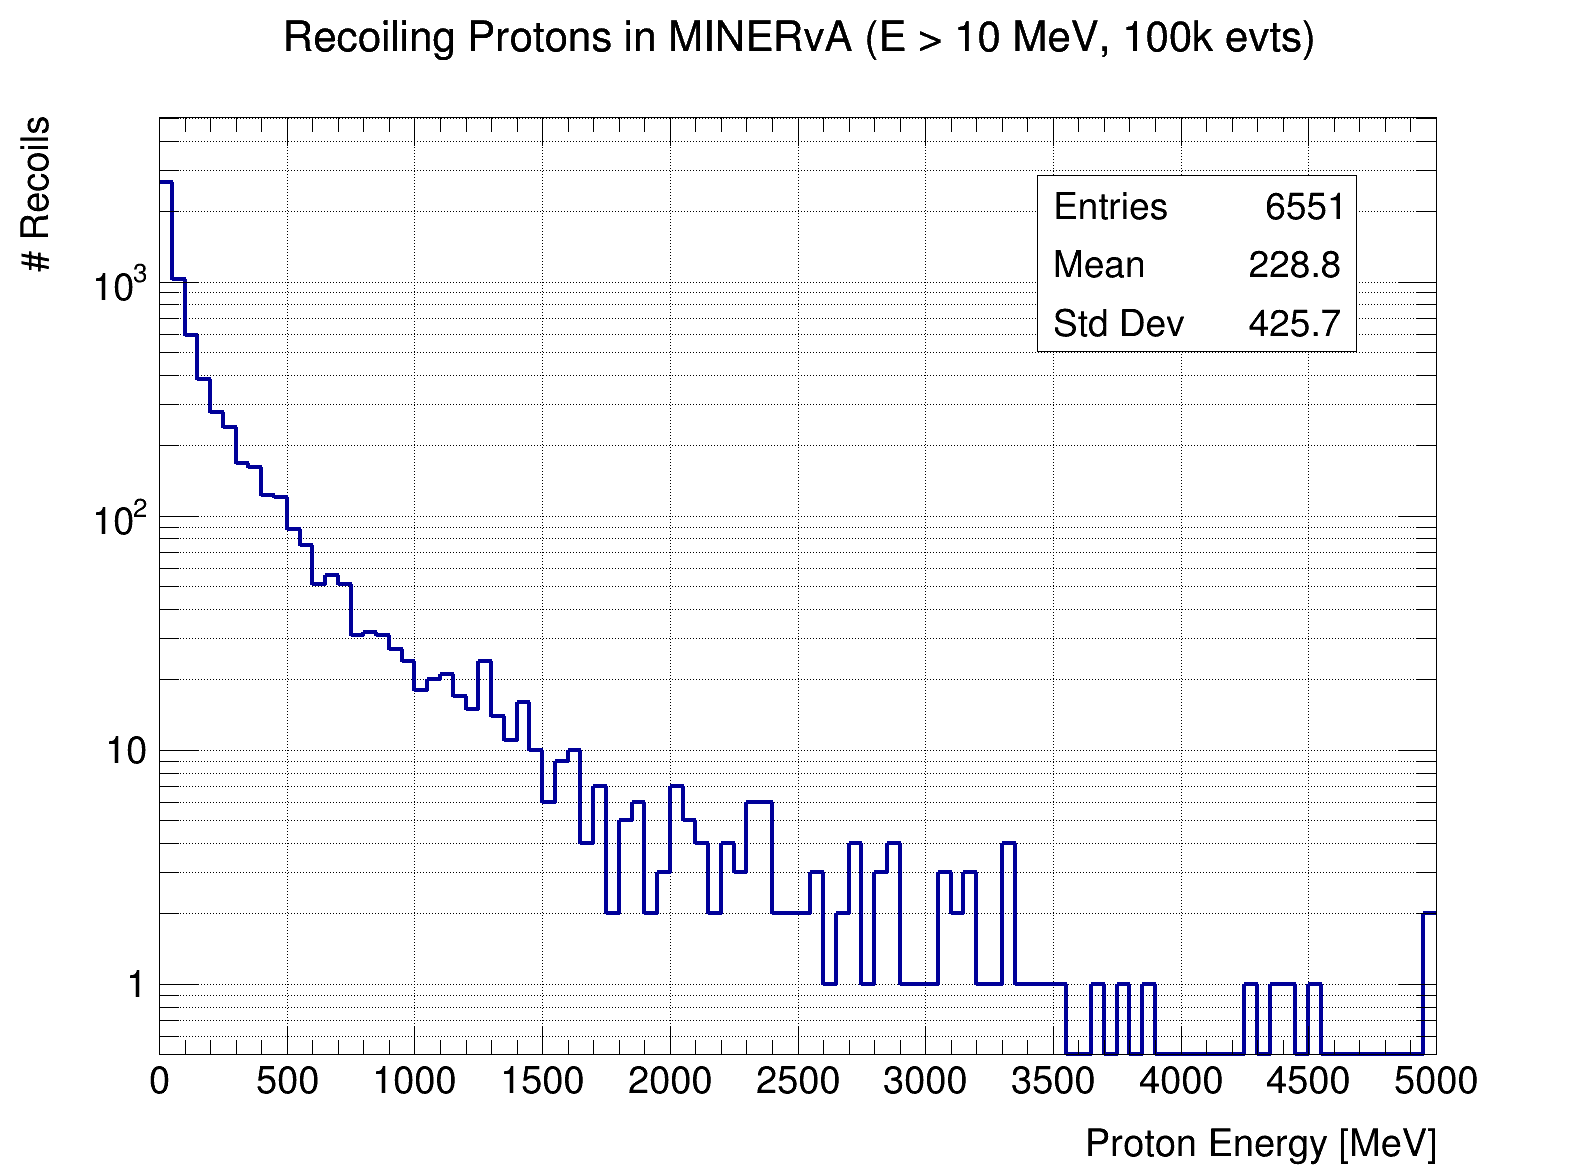
\includegraphics[width=0.45\textwidth]{plots/2x2_minerva_plots/recoils_vs_E_proton_MINERvA.png}}
  \caption{}
  \label{fig:neutron_tag_minerva}
\end{figure}

\FloatBarrier
\subsection{Repurposing the MINOS Near Detector}

%We note that the configuration discussed here may not be optimal. Some of the MINERvA scintillator modules could be used to provide vetos for particles entering or exiting the 2x2 cryostat, or to contain side-escaping showers. Indeed, the optimal design would also depend on whether use of the MINOS near detector as part of the ProtoDUNE-ND setup were supported. Here we discuss such possibilities in brief, and will wait to discover the viability of this project before embarking on more detailed studies.

\todo{the following needs expanding from notes, and making consistent with the above}

The MINOS ND~\cite{MINOS_NIM} is a magnetic spectrometer formed of \SI{1}{\kilo\tonne} of steel and plastic scintillator.
It is located \SI{2.1}{\metre} downstream of MINERvA in the NuMI beam line. 

A schematic of MINOS ND is shown in Figure~\ref{fig:minos_near_detector}, it consists of 282 planes of \SI{2.54}{\centi\metre} thick steel. Only 152 planes are instrumented with scintillator. Each scintillator plane is made of \SI{1}{\centi\metre} thick  and \SI{4.1}{\centi\metre} wide strips. 
The 120 most upstream planes form the calorimeter region, partially-instrumented scintillator planes separate steel planes, with only every fifth plane fully-instrumented. Downstream, the remaining 162 planes form the muon spectrometer, there are no partially instrumented planes and every fifth plane has full scintillator coverage. 

\begin{figure}[htb]
	\centering
	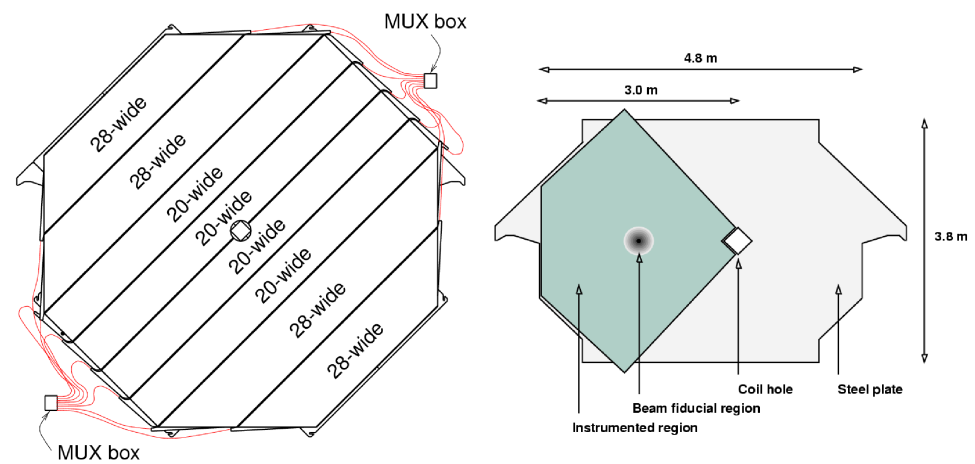
\includegraphics[width=0.9\textwidth]{plots/minos.png}
	\caption{Left: Top view of the MINOS near detector, showing the calorimeter and muon spectrometer (not to scale). Right: transverse view of a near detector plane. The shaded area shows a partially instrumented active scintillator plane and the dashed line within shows the boundary of the fiducial region. The dotted line shows the outline of a fully instrumented scintillator plane. Taken from Figure~2 of~\cite{MINOSDetectors}.}
	\label{fig:minos_near_detector}
\end{figure}

Employing MINOS ND as a range finder will allow for the augmentation of MINERvA, since the entire MINERvA detector would no longer be needed downstream to maximise momentum sensitivity.
MINERvA EM scintillator modules could be used to provide vetos for cosmic and rock induced particles entering or exiting the 2x2 cryostat, or to contain side-escaping showers. 
This would enable a test of the assumption that the DUNE ND does not require a side muon tracker. 
Here we discuss such possibilities in brief, and will wait to discover the viability of this project before embarking on more detailed studies.
Use of the MINOS ND, in combination with an augmented MINERvA, will allow the reconstruction of the entire properties of an event within 2x2.
This serves as a proxy for neutrino energy reconstruction, and provides the most thorough calibration of the response of 2x2.  

\subsubsection{Validation of multiple coulomb scattering}

\subsubsection{Use as a cosmic trigger}
\todo{Move some stuff from previous sections for this.}
